% SPDX-License-Identifier: CC-BY-SA-4.0
% Author: Matthieu Perrin
% Part: 
% Section: 
% Sub-section: 
% Frame: 

\begingroup

\begin{frame}{Ambiguité, priorité, associativité}

  \begin{block}{Définition -- ambiguïté}
    Une grammaire est ambiguë si deux arbres de dérivation génèrent le même mot.
    \example{Exemple : }   $\left\{\begin{array}{rcl} A & \rightarrow & A \oplus A | A \otimes A | a \end{array}\right.$
  \end{block}
  
  \uncover<2->{
    \structure{Comment régler les principales causes d'ambiguïté ?}
    \begin{itemize}
    \item $\oplus$ est associatif à gauche quand : \hspace\fill $x \oplus y \oplus z$ signifie $(x \oplus y) \oplus z$\\
      \example{Exemple : } \lstinline{4 - 2 - 1}
      
    \item<3-> $\oplus$ est associatif à droite quand : \hspace\fill $x \oplus y \oplus z$ signifie $x \oplus (y \oplus z)$\\
      \example{Exemple : } \lstinline{x = y = 0;}
      
    \item<4-> $\otimes$ est prioritaire sur $\oplus$ quand : \hspace\fill $w \otimes x \oplus y \otimes z$ signifie $(w \otimes x) \oplus (y \otimes z)$\\
      \example{Exemple : } \lstinline{3 * 5 + 2}
      
    \end{itemize}
  }

  \uncover<2->{
    \begin{minipage}[t]{.33\textwidth}
      \structure{Associativité à gauche :}\\
      
      \centering

      $\left\{\begin{array}{rcl}
      A & \rightarrow & A \oplus B | B 
      \end{array}\right.$
      
      \centering
      \scalebox{.7}{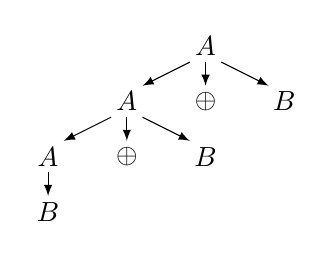
\begin{tikzpicture}
          \draw (5,7.1) node{$A$};
          \draw (4,6.4) node{$A$};
          \draw (5,6.4) node{$\oplus$};
          \draw (6,6.4) node{$B$};
          \draw (3,5.7) node{$A$};
          \draw (4,5.7) node{$\oplus$};
          \draw (5,5.7) node{$B$};
          \draw (3,5.0) node{$B$};

          \draw[-latex] (4.8,6.9) -- (4.2,6.6); 
          \draw[-latex] (5.0,6.9) -- (5.0,6.6); 
          \draw[-latex] (5.2,6.9) -- (5.8,6.6); 
          \draw[-latex] (3.8,6.2) -- (3.2,5.9); 
          \draw[-latex] (4.0,6.2) -- (4.0,5.9); 
          \draw[-latex] (4.2,6.2) -- (4.8,5.9); 
          \draw[-latex] (3.0,5.5) -- (3.0,5.2); 
      \end{tikzpicture}}
  \end{minipage}}%
  \uncover<3->{\begin{minipage}[t]{.33\textwidth}
      \structure{Associativité à droite :}\\

      $\left\{\begin{array}{rcl}
      A & \rightarrow & B \oplus A | B 
      \end{array}\right.$
      
      \centering
      \scalebox{.7}{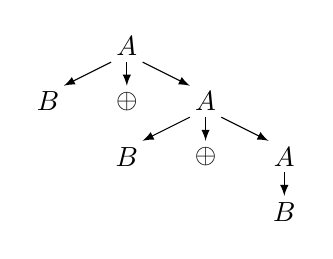
\begin{tikzpicture}
          \draw (5,7.1) node{$A$};
          \draw (4,6.4) node{$B$};
          \draw (5,6.4) node{$\oplus$};
          \draw (6,6.4) node{$A$};
          \draw (5,5.7) node{$B$};
          \draw (6,5.7) node{$\oplus$};
          \draw (7,5.7) node{$A$};
          \draw (7,5.0) node{$B$};

          \draw[-latex] (4.8,6.9) -- (4.2,6.6); 
          \draw[-latex] (5.0,6.9) -- (5.0,6.6); 
          \draw[-latex] (5.2,6.9) -- (5.8,6.6); 
          \draw[-latex] (5.8,6.2) -- (5.2,5.9); 
          \draw[-latex] (6.0,6.2) -- (6.0,5.9); 
          \draw[-latex] (6.2,6.2) -- (6.8,5.9); 
          \draw[-latex] (7.0,5.5) -- (7.0,5.2); 
      \end{tikzpicture}}
  \end{minipage}}%
  \uncover<4->{\begin{minipage}[t]{.33\textwidth}
      \structure{Priorité :}\\

      $\left\{\begin{array}{rcl}
      A & \rightarrow & B \oplus B | B \\
      B & \rightarrow & C \otimes C | C 
      \end{array}\right.$
      
      \centering
      \scalebox{.7}{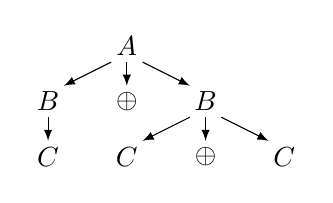
\begin{tikzpicture}
          \draw (5,7.1) node{$A$};
          \draw (4,6.4) node{$B$};
          \draw (5,6.4) node{$\oplus$};
          \draw (6,6.4) node{$B$};
          \draw (4,5.7) node{$C$};
          \draw (5,5.7) node{$C$};
          \draw (6,5.7) node{$\oplus$};
          \draw (7,5.7) node{$C$};

          \draw[-latex] (4.8,6.9) -- (4.2,6.6); 
          \draw[-latex] (5.0,6.9) -- (5.0,6.6); 
          \draw[-latex] (5.2,6.9) -- (5.8,6.6); 
          \draw[-latex] (5.8,6.2) -- (5.2,5.9); 
          \draw[-latex] (6.0,6.2) -- (6.0,5.9); 
          \draw[-latex] (6.2,6.2) -- (6.8,5.9); 
          \draw[-latex] (4.0,6.2) -- (4.0,5.9); 
      \end{tikzpicture}}
  \end{minipage}}%
\end{frame}

\endgroup
